% ============================================================================
% CHAPTER I: OVERVIEW OF EMBEDDED SYSTEMS
% Academic & Technical Presentation (LaTeX Beamer)
% Exact style match with Chapter II:
% - Template background: figs/bg.jpg (Cyan top banner + PTIT logo + 16:9 white body)
% - Minimal flat layout: NO cards, NO bounding boxes, NO shadows
% - Latin Modern font (\usepackage{lmodern})
% - Text & bullets directly on white background
% ============================================================================
\documentclass[aspectratio=169]{beamer}

\usepackage[T1]{fontenc}
\usepackage[utf8]{inputenc}
\usepackage{lmodern}
\usepackage{graphicx}
\usepackage{xcolor}
\usepackage{tikz}
\usepackage{booktabs}
\usepackage{array}

\definecolor{ptitblue}{HTML}{00A9CE}
\setbeamertemplate{navigation symbols}{}
\setbeamertemplate{footline}{%
  \hfill{\color{gray}\footnotesize\insertframenumber}\hspace{0.4cm}\vspace{0.25cm}}
\setbeamertemplate{background}{%
  
\includegraphics[width=\paperwidth,height=\paperheight]{figs/bg.jpg}}
\setbeamertemplate{itemize item}{\color{ptitblue}$\blacktriangleright$}
\setbeamertemplate{itemize subitem}{\color{ptitblue}--}
\setlength{\leftmargini}{0.55cm}
\setlength{\itemsep}{0.35cm}

% Slide title inside cyan banner (matches Chapter II)
\newcommand{\slidetitle}[1]{%
  \begin{tikzpicture}[remember picture,overlay]
    \node[anchor=west, text=white, font=\bfseries\fontsize{17}{21}\selectfont,
      text width=0.82\paperwidth, inner sep=0pt]
      at ([xshift=0.5cm,yshift=-0.58cm]current page.north west) {\uppercase{#1}};
  \end{tikzpicture}%
  \vspace*{1.55cm}}

% Left column figure with caption
\newcommand{\leftfig}[2]{%
  \includegraphics[width=\linewidth]{#1}\\[0.15cm]
  {\footnotesize\color{black!70}\textit{#2}}}

\begin{document}

% ===================== 1. TITLE SLIDE =====================
\begin{frame}[plain,t]
  \slidetitle{CHAPTER I. OVERVIEW OF EMBEDDED SYSTEMS}
  \par\vspace{0.1cm}
  \begin{columns}[T]
    \column{0.60\textwidth}
      {\normalsize\textbf{Foundations, Core Characteristics \& Software Architecture}}\\[0.25cm]
      \begin{itemize}
        \item \textbf{Curriculum Scope:} Core Embedded Systems \& Edge Computing Architecture
        \item \textbf{Engineering Paradigms:} Deep hardware-software co-design, deterministic timing, and tight resource budgets
        \item \textbf{Target Platform:} 32-bit Microcontroller Core (ARM Cortex-M85 / Renesas RA8M1)
        \item \textbf{Implementation Standards:} C99/POSIX firmware patterns, Hard RTOS, standardized MCAL/HAL stacks
      \end{itemize}
    \column{0.38\textwidth}
      \begin{center}
      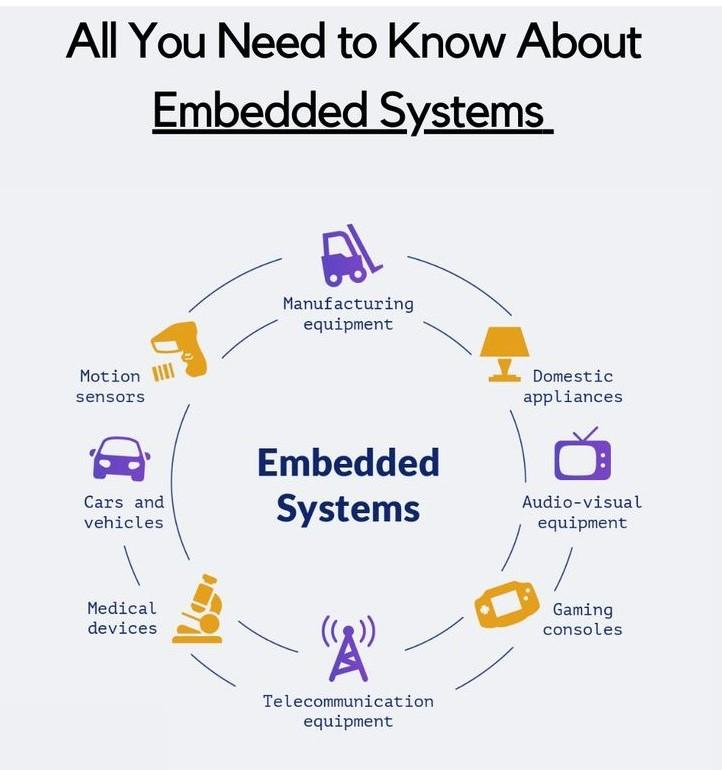
\includegraphics[height=5.2cm]{figs/fig_cover.jpg}
      \end{center}
  \end{columns}
\end{frame}

% ===================== 2. TABLE OF CONTENTS =====================
\begin{frame}[plain,t]
  \slidetitle{TABLE OF CONTENTS}
  \par\vspace{0.05cm}
  {\normalsize\textbf{1. Concept \& Nature of Embedded Systems}}\\[0.05cm]
  {\footnotesize\hspace{0.8cm}1.1. Standard Definition, 3-Element Triad, and Physical Embedded Nature\\
  \hspace{0.8cm}1.2. Role of Embedded Systems in IoT \& Edge Computing}\\[0.15cm]
  {\normalsize\textbf{2. Core Technical Characteristics}}\\[0.05cm]
  {\footnotesize\hspace{0.8cm}2.1. Dedicated Functionality \& Severe Resource Constraints\\
  \hspace{0.8cm}2.2. Deterministic Real-Time Execution \& High Reliability (WDT, BOD, CRC)\\
  \hspace{0.8cm}2.3. Ultra-Low Power, Embedded Security \& Firmware Maintenance (OTA)}\\[0.15cm]
  {\normalsize\textbf{3. Embedded Systems vs. General-Purpose Computers}}\\[0.05cm]
  {\footnotesize\hspace{0.8cm}3.1. Architectural Paradigms: Specialization vs. Versatility\\
  \hspace{0.8cm}3.2. Detailed Multi-Criteria Technical Comparison Matrix}\\[0.15cm]
  {\normalsize\textbf{4. Layered Embedded Software Architecture}}\\[0.05cm]
  {\footnotesize\hspace{0.8cm}4.1. The 5-Layer Stack Model: Hardware $\rightarrow$ MCAL $\rightarrow$ HAL $\rightarrow$ RTOS $\rightarrow$ Middleware $\rightarrow$ Application\\
  \hspace{0.8cm}4.2. RTOS Layer: Multitasking vs. Super-Loop \& Inter-Process Communication\\
  \hspace{0.8cm}4.3. Middleware \& Application Layer: Decoupling and Host Testability}\\[0.22cm]
  \textbf{$\Rightarrow$ Guiding Question: What fundamentally distinguishes embedded software from desktop/PC software?}
\end{frame}

% ===================== 3. DEFINITION & NATURE =====================
\begin{frame}
  \slidetitle{1.1. Embedded System Definition \& Nature}
  \begin{columns}[T]
    \column{0.49\textwidth}
      \leftfig{figs/fig_1_1_typical_system.jpg}{Figure 1.1: Architecture of a Typical Embedded System}
    \column{0.49\textwidth}
      \begin{itemize}
        \item \textbf{Definition:} Specialized computer system integrated within a host device to perform dedicated, pre-defined functions.
        \item \textbf{Triad Nature:} Inseparable co-design between \textbf{Computation} (Hardware) --- \textbf{Processing Logic} (Firmware) --- \textbf{Physical World Interaction} (Sensors/Actuators).
        \item \textbf{Design Goal:} Fulfill dedicated tasks under strict constraints: deterministic latency, ultra-low power, compact size, high MTBF, and low unit cost.
        \item \textbf{Distinction:} Not a general-purpose PC --- strictly eliminates software bloat in favor of deep optimization for a single mission.
        \item \textbf{Real Example:} Environmental monitoring edge node: continuous sensing, local anomaly detection, and 24/7 telemetry.
      \end{itemize}
  \end{columns}
\end{frame}

% ===================== 4. HARDWARE SUBSYSTEMS =====================
\begin{frame}
  \slidetitle{1.1. Hardware Architecture \& Subsystems}
  \begin{columns}[T]
    \column{0.49\textwidth}
      \leftfig{figs/fig_1_1_2_hardware.jpg}{Figure 1.2: Hardware Subsystems of an Embedded Device}
    \column{0.49\textwidth}
      \begin{itemize}
        \item \textbf{Core Processing (MCU):} Silicon microcontroller integrating CPU core, hardware timers, DMA controllers, and low-latency NVIC.
        \item \textbf{Memory Hierarchy:} Embedded \textbf{Flash Memory} for persistent firmware; tight on-chip \textbf{SRAM} for execution stack, heap, and buffers.
        \item \textbf{Physical Transducers:} High-precision \textbf{Sensors} paired with robust \textbf{Actuators} (relays, buzzers, solenoid valves).
        \item \textbf{Communication Buses:} Local serial interfaces (\textbf{UART, SPI, I2C, CAN}) alongside networked transceivers (\textbf{Ethernet, Wi-Fi, Cellular}).
        \item \textbf{Power \& Protection:} Integrated \textbf{LDO} regulators, Brown-Out Detector (\textbf{BOD}), and hardware \textbf{Watchdog Timers}.
      \end{itemize}
  \end{columns}
\end{frame}

% ===================== 5. EDGE COMPUTING IN IOT =====================
\begin{frame}
  \slidetitle{1.1. Embedded Nature \& Edge Computing in IoT}
  \begin{columns}[T]
    \column{0.49\textwidth}
      \leftfig{figs/fig_1_1_3_edge.png}{Figure 1.3: Embedded Edge Node in Cloud-IoT Topology}
    \column{0.49\textwidth}
      \begin{itemize}
        \item \textbf{The `Embedded' Nature:} Deeply encapsulated inside host machinery; user interacts solely via HMI or cloud; requires bare-metal register manipulation.
        \item \textbf{Frontline IoT Edge Node:} Serves as the vital physical bridge collecting field telemetry and driving deterministic real-time actuation.
        \item \textbf{On-Device Edge Computing:} Performs local filtering, anomaly classification, and inference at the edge, drastically reducing cloud bandwidth and latency.
        \item \textbf{Disconnection Resilience:} Operates 100\% autonomously during WAN network blackouts; maintains local safety cutoffs independently.
        \item \textbf{Data Fallback:} Retains critical telemetry on local SD/Flash memory during signal loss and automatically synchronizes upon reconnection.
      \end{itemize}
  \end{columns}
\end{frame}

% ===================== 6. RESOURCE CONSTRAINTS =====================
\begin{frame}
  \slidetitle{1.2. Dedicated Functionality \& Resource Constraints}
  \begin{columns}[T]
    \column{0.49\textwidth}
      \leftfig{figs/fig_1_2_characteristics.jpg}{Figure 1.4: Multi-dimensional Constraints in Embedded Design}
    \column{0.49\textwidth}
      \begin{itemize}
        \item \textbf{Dedicated Functionality:} Hardware and firmware are strictly trimmed to the target workload $\rightarrow$ minimizes BOM unit cost and eliminates software bloat.
        \item \textbf{Engineering Trade-off:} High specialization reduces generic software reusability; major specification shifts necessitate PCB redesign.
        \item \textbf{Scarce Flash Memory:} Constrained to tens of KB to few MB (vs. hundreds of GB SSD on PCs) $\rightarrow$ demands aggressive code footprint minimization.
        \item \textbf{Extremely Tight SRAM:} Limited to 16 KB -- 512 KB $\rightarrow$ \textbf{dynamic heap allocation (\texttt{malloc}) is strictly prohibited}; static allocation is mandatory.
        \item \textbf{Clock Speed \& Pinout:} Conservative MHz clock rates to conserve battery; tightly budgeted GPIO pinout requires pin multiplexing.
      \end{itemize}
  \end{columns}
\end{frame}

% ===================== 7. REAL-TIME DETERMINISM & RELIABILITY =====================
\begin{frame}
  \slidetitle{1.2. Real-Time Determinism \& System Reliability}
  \begin{columns}[T]
    \column{0.49\textwidth}
      {\normalsize\textbf{Real-Time Determinism \& Deadlines}}\\[0.15cm]
      \begin{itemize}
        \item \textbf{Correctness Criteria:} System correctness requires \textbf{both} logical accuracy AND completion strictly before defined \textbf{Deadlines}.
        \item \textbf{Hard Real-Time:} Missing a deadline causes catastrophic destruction or loss of human life (\textit{airbags, ABS braking, medical ventilators}).
        \item \textbf{Soft Real-Time:} Deadline misses degrade Quality of Service without catastrophic harm (\textit{UI display refresh, periodic logging}).
        \item \textbf{Deterministic Timing:} Interrupt latency and execution times must have mathematical upper bounds; zero tolerance for unbounded jitter.
        \item \textbf{Architectural Support:} Enforced via low-latency NVIC and preemptive priority RTOS scheduling.
      \end{itemize}
    \column{0.49\textwidth}
      {\normalsize\textbf{Autonomous Reliability \& Self-Healing}}\\[0.15cm]
      \begin{itemize}
        \item \textbf{Continuous 24/7 Uptime:} Must operate unattended for decades without human manual intervention or reboot.
        \item \textbf{Watchdog Timer (WDT):} Independent free-running counter resets the MCU automatically if firmware deadlocks or enters an infinite loop.
        \item \textbf{Brown-Out Detector (BOD):} Continually monitors supply voltage droop, forcing safe reset before Flash memory is corrupted.
        \item \textbf{CRC Integrity:} Hardware CRC engine verifies Flash code integrity and communication packet validity.
        \item \textbf{Fail-Safe Defaults:} Automatic fallback into safe benign states (\textit{opening relays, sounding alarms}) upon critical faults.
      \end{itemize}
  \end{columns}
\end{frame}

% ===================== 8. POWER & SECURITY =====================
\begin{frame}
  \slidetitle{1.2. Power Efficiency, Security \& Maintenance}
  \begin{columns}[T]
    \column{0.49\textwidth}
      {\normalsize\textbf{Ultra-Low Power Optimization}}\\[0.15cm]
      \begin{itemize}
        \item \textbf{Deep Sleep States:} Advanced low-power modes (Sleep, Standby, Deep Software Standby) dropping quiescent current to microamperes ($\mu\text{A}$).
        \item \textbf{Interrupt-Driven Wakeup:} CPU core remains powered down, waking up solely upon external sensor edge interrupts or periodic RTC timers.
        \item \textbf{Autonomous DMA Transfers:} Direct Memory Access transfers peripheral data to RAM buffers without CPU intervention, maximizing sleep duty cycles.
        \item \textbf{Energy Harvesting:} Supports ultra-low-power duty cycles compatible with solar, thermal, and RF energy-harvesting nodes.
      \end{itemize}
    \column{0.49\textwidth}
      {\normalsize\textbf{Embedded Security \& Maintenance}}\\[0.15cm]
      \begin{itemize}
        \item \textbf{Hardware Secure Boot:} Silicon cryptographic engine validates digital signatures (RSA/ECC) of firmware before allowing boot execution.
        \item \textbf{Arm TrustZone Isolation:} Partitions memory and peripherals into Secure and Non-Secure domains, isolating encryption keys from user code.
        \item \textbf{Line-Rate Encryption:} Hardware-accelerated AES, SHA-256, and ECC engines enable secure TLS/DTLS encryption for cloud telemetry.
        \item \textbf{Dual-Bank Flash OTA:} Downloads and stages new firmware images into secondary Flash bank without downtime; automated rollback on failure.
      \end{itemize}
  \end{columns}
\end{frame}

% ===================== 9. GPC VS EMBEDDED =====================
\begin{frame}
  \slidetitle{1.3. Embedded Systems vs. General-Purpose PCs}
  \begin{columns}[T]
    \column{0.49\textwidth}
      \leftfig{figs/fig_1_3_gpc_vs_embedded.jpg}{Figure 1.5: Paradigm Comparison: General-Purpose PC vs. Embedded System}
    \column{0.49\textwidth}
      \begin{itemize}
        \item \textbf{Specialization vs. Versatility:} General-Purpose Computers (GPC) run arbitrary multi-user software, office suites, and gaming. Embedded systems are deeply pruned for one dedicated workload.
        \item \textbf{Monolithic SoC Integration:} Embedded MCUs integrate CPU, SRAM, Flash ROM, ADC/DAC, timers, and serial controllers on a single die. PCs rely on discrete motherboards with socketed CPUs and RAM sticks.
        \item \textbf{Environmental Robustness:} Embedded systems survive extreme industrial temperatures ($-40^\circ\text{C}$ to $+85^\circ\text{C}$ / $125^\circ\text{C}$), high vibration, dust, and electrical noise. PCs require climate-controlled rooms and active fans.
        \item \textbf{Cost \& Unit Optimization:} MCU Bill-of-Materials cost is measured in single-digit dollars for mass production, whereas PC platforms cost hundreds to thousands of dollars.
      \end{itemize}
  \end{columns}
\end{frame}

% ===================== 10. COMPARISON MATRIX =====================
\begin{frame}
  \slidetitle{1.3. Detailed Technical Comparison Matrix}
  \vspace{0.15cm}
  \begin{center}
  {\footnotesize
  \setlength{\tabcolsep}{5pt}
  \renewcommand{\arraystretch}{1.15}
  \begin{tabular}{p{0.22\textwidth}p{0.36\textwidth}p{0.36\textwidth}}
    \toprule
    \textbf{Evaluation Metric} & \textbf{Embedded Systems (MCU-based)} & \textbf{General-Purpose Computers (PC-based)} \\
    \midrule
    Design Objective & Dedicated, deeply optimized for a single mission & Versatile, executes arbitrary concurrent user applications \\
    Processor Core & Low-power MCU (e.g., ARM Cortex-M), SoC, DSP (MHz) & High-speed multi-core CPU (x86/x64, GHz), discrete GPU \\
    Memory Hierarchy & Flash: 32 KB -- 4 MB; SRAM: 8 KB -- 1 MB (On-chip) & RAM: 8 GB -- 64+ GB; Storage: 512 GB -- Multiple TB SSD \\
    Operating System & Bare-metal firmware, Hard RTOS (\textit{FreeRTOS, Zephyr}) & General-Purpose OS (\textit{Windows, Linux, macOS}) \\
    Timing Constraints & Deterministic hard/soft real-time; bounded $\mu$s latency & Best-effort execution; non-deterministic task scheduling \\
    Power Consumption & Ultra-low power (mW to $\mu$A); multi-year battery operation & High power draw (50W -- 500W+); continuous AC mains \\
    Operating Environment & Harsh industrial ($-40^\circ\text{C}$ to $85^\circ\text{C}$), vibration, dust & Benign indoor climate; office/datacenter environments \\
    Maintenance & Secure remote OTA firmware; decades-long operational life & Frequent OS patches, dynamic package installations \\
    \bottomrule
  \end{tabular}}
  \end{center}
  \vspace{0.1cm}
  \textbf{$\Rightarrow$ Conclusion:} For dedicated IoT edge monitoring, specialized MCUs (Cortex-M85 / RA8M1) vastly outperform PCs in determinism, reliability, power efficiency, and unit cost.
\end{frame}

% ===================== 11. 5-LAYER ARCHITECTURE =====================
\begin{frame}
  \slidetitle{1.4. The 5-Layer Embedded Software Architecture}
  \begin{columns}[T]
    \column{0.49\textwidth}
      \leftfig{figs/fig_1_4_layered_arch.jpg}{Figure 1.6: Standard 5-Layer Embedded Software Stack}
    \column{0.49\textwidth}
      \begin{itemize}
        \item \textbf{Separation of Concerns:} Each architectural tier encapsulates specific functional responsibilities, hiding lower-level hardware quirks from upper layers.
        \item \textbf{Hardware Decoupling:} Application logic never manipulates raw chip registers; all hardware interactions pass through standardized APIs.
        \item \textbf{Concurrent Engineering:} Hardware schematics and software develop in parallel; allows extensive Unit Testing natively on host PCs.
        \item \textbf{Silicon Portability:} When migrating to an alternative MCU vendor, only the MCAL/HAL drivers are rewritten---preserving \textbf{100\% of Middleware and Application code}.
        \item \textbf{Extensibility:} Modifying hardware components (\textit{e.g., swapping an analog sensor for an I2C sensor}) requires zero changes to core business rules.
      \end{itemize}
  \end{columns}
\end{frame}

% ===================== 12. HARDWARE & MCAL / HAL =====================
\begin{frame}
  \slidetitle{1.4.1 -- 1.4.2. Hardware Layer \& MCAL / HAL}
  \begin{columns}[T]
    \column{0.49\textwidth}
      {\normalsize\textbf{Physical Hardware Layer}}\\[0.15cm]
      \begin{itemize}
        \item \textbf{Target Silicon:} MCU silicon (e.g., Renesas RA8M1 / Cortex-M85), analog front-ends, relay drivers, communication transceivers.
        \item \textbf{PCB Layout Integrity:} Physical trace routing directly dictates Signal-to-Noise Ratio (SNR), ADC sampling precision, and parasitic leakage currents.
        \item \textbf{Hardware Robustness:} In-line PTC resettable fuses, TVS suppression diodes, and galvanic isolation prevent field electrical destruction.
        \item \textbf{Engineering Reality:} Silicon layout bugs and hardware flaws cannot be solved by software patches alone---demands rigorous design validation.
      \end{itemize}
    \column{0.49\textwidth}
      {\normalsize\textbf{MCAL vs. HAL Driver Layers}}\\[0.15cm]
      \begin{itemize}
        \item \textbf{MCAL (Microcontroller Abstraction):} Hardware-dependent register manipulation; configures internal silicon clocks, pin multiplexing, interrupt routing, and DMA channels.
        \item \textbf{HAL (Hardware Abstraction Layer):} Vendor-neutral API abstraction wrapping register complexity into uniform C calls (\texttt{HAL\_GPIO\_WritePin()}, \texttt{HAL\_ADC\_Read()}).
        \item \textbf{Device Driver Interface:} Provides standard bus interfaces allowing external sensor/actuator drivers to operate seamlessly across different chips.
        \item \textbf{Portability Boundary:} Decouples silicon-specific CMSIS headers from higher-level middleware and application stacks.
      \end{itemize}
  \end{columns}
\end{frame}

% ===================== 13. RTOS LAYER =====================
\begin{frame}
  \slidetitle{1.4.3. Real-Time Operating System (RTOS Layer)}
  \begin{columns}[T]
    \column{0.49\textwidth}
      {\normalsize\textbf{Preemptive Multitasking vs. Super-Loop}}\\[0.15cm]
      \begin{itemize}
        \item \textbf{Super-Loop Pitfalls:} Sequential \texttt{while(1)} polling suffers catastrophic latency blockage when long I/O tasks (\textit{e.g., TCP network handshakes}) stall the CPU.
        \item \textbf{Preemptive Priority Scheduling:} Critical high-priority tasks (\textit{e.g., fire detection, over-temperature alarm}) preempt the CPU within microseconds upon interrupt.
        \item \textbf{Deterministic Software Timers:} Non-blocking software timers drive periodic sensor acquisitions with millisecond determinism.
        \item \textbf{Tickless Low-Power Idle:} Automatically transitions the MCU core into deep sleep whenever all tasks are blocked in wait states.
      \end{itemize}
    \column{0.49\textwidth}
      {\normalsize\textbf{IPC \& Resource Synchronization}}\\[0.15cm]
      \begin{itemize}
        \item \textbf{Message Queues:} Safe FIFO message queues pass sensor telemetry to processing tasks without memory corruption or locks.
        \item \textbf{Mutexes \& Semaphores:} Guard shared communication buses (\textit{I2C, SPI, UART}) against race conditions and priority inversions.
        \item \textbf{Task Priority Hierarchy:} Emergency Safety Alarms (High) $\rightarrow$ Sensor Filtering (Medium) $\rightarrow$ Cloud MQTT Telemetry (Low).
        \item \textbf{Leading Industrial RTOS:} \textbf{FreeRTOS} (ubiquitous, minimal footprint), \textbf{Zephyr RTOS} (modular, modern IoT stack), \textbf{Azure RTOS / ThreadX}.
      \end{itemize}
  \end{columns}
\end{frame}

% ===================== 14. MIDDLEWARE LAYER =====================
\begin{frame}
  \slidetitle{1.4.4. Middleware \& System Services Layer}
  \begin{columns}[T]
    \column{0.49\textwidth}
      {\normalsize\textbf{IoT Networking \& Protocol Stacks}}\\[0.15cm]
      \begin{itemize}
        \item \textbf{Embedded TCP/IP Stack:} Lightweight network stacks (\textbf{LwIP}, FreeRTOS-Plus-TCP) powering low-overhead Ethernet and Wi-Fi connectivity.
        \item \textbf{MQTT Protocol:} Lightweight Publish/Subscribe messaging protocol minimizing transmission packet overhead and radio active time.
        \item \textbf{CoAP \& HTTP Micro-Servers:} Embedded micro-web servers for on-site device commissioning, status diagnostics, and RESTful APIs.
        \item \textbf{DHCP \& DNS Clients:} Automated IP dynamic configuration and central cloud hostname resolution over dynamic local networks.
      \end{itemize}
    \column{0.49\textwidth}
      {\normalsize\textbf{Security, Storage \& Maintenance}}\\[0.15cm]
      \begin{itemize}
        \item \textbf{Cryptographic Library (MbedTLS):} Implements industry-grade TLS 1.3 / DTLS encryption, safeguarding telemetry against eavesdropping and MITM attacks.
        \item \textbf{Embedded File System (FatFS):} Hardware-independent FAT12/16/32 and exFAT implementation for local microSD and external SPI Flash storage.
        \item \textbf{Robust OTA Engine:} Handles remote firmware download, cryptographic hash validation (SHA-256), and dual-bank Flash staging.
        \item \textbf{Diagnostics \& Logging:} Tracks runtime CPU load, stack watermarks, memory leaks, and records multi-level error logs for post-mortem analysis.
      \end{itemize}
  \end{columns}
\end{frame}

% ===================== 15. APPLICATION LAYER =====================
\begin{frame}
  \slidetitle{1.4.5. Application Layer \& Domain Logic}
  \begin{columns}[T]
    \column{0.49\textwidth}
      {\normalsize\textbf{Core Domain Tasks \& Signal Processing}}\\[0.15cm]
      \begin{itemize}
        \item \textbf{Periodic Sampling:} Orchestrates multi-sensor data acquisition (ambient temperature, relative humidity, VOC/toxic gas, structural vibration).
        \item \textbf{Digital Signal Processing:} Implements Moving Average or Kalman filters to eliminate electrical noise spikes and sensor drift.
        \item \textbf{Threshold Evaluation:} Classifies environmental health across multi-tiered levels: Normal $\rightarrow$ Warning $\rightarrow$ Critical Alarm.
        \item \textbf{Autonomous Emergency Actuation:} Drives safety actuators immediately upon anomaly detection (\textit{opening relays, running fans, sirens}).
        \item \textbf{Telemetry Serialization:} Encodes validated telemetry into compact standard formats (\textit{JSON, CBOR, Protocol Buffers}).
      \end{itemize}
    \column{0.49\textwidth}
      {\normalsize\textbf{Design Decoupling \& Host Testability}}\\[0.15cm]
      \begin{itemize}
        \item \textbf{Total Hardware Independence:} Pure business logic interacts strictly through generic domain APIs (\texttt{get\_sensor\_data()}, \texttt{trigger\_alarm()}).
        \item \textbf{Transducer Modularity:} Replacing an analog sensor with an I2C sensor leaves 100% of threshold comparison logic completely untouched.
        \item \textbf{Host-Based Simulation:} Entire application state machine compiles and runs on a host PC using simulated sensor streams for rapid verification.
        \item \textbf{Finite State Machine (FSM):} Structured as deterministic states: Boot $\rightarrow$ Normal Operation $\rightarrow$ Warning $\rightarrow$ Emergency Fault.
      \end{itemize}
  \end{columns}
\end{frame}

% ===================== 16. CHAPTER SUMMARY =====================
\begin{frame}
  \slidetitle{Chapter I Summary \& Transition to Chapter II}
  \begin{itemize}
    \item \textbf{Embedded Co-Design:} Tight synergy between specialized MCU silicon, deterministic firmware, and physical world transducers.
    \item \textbf{The Core Triad:} Stringent resource boundaries, deterministic real-time deadlines, and 24/7 unassisted autonomous reliability.
    \item \textbf{The 5-Layer Stack:} Golden architectural standard separating silicon registers from business logic, ensuring portability and maintainability.
    \item \textbf{Escalating Edge Demands:} Modern IoT edge stations demand on-device ML/DSP, sub-microsecond interrupt latency, and silicon-enforced domain security.
    \item \textbf{Bridge to Chapter II:} Transitioning from legacy 8/16-bit or basic 32-bit cores to advanced vector-accelerated architectures.
  \end{itemize}
  \vspace{0.35cm}
  \textbf{$\Rightarrow$ Chapter II: Embedded Processor Architectures \& ARM Cortex-M85 on Renesas RA8M1.}
\end{frame}

\end{document}
